%\documentclass[11pt,hyperref={bookmarks=false}]{beamer}
%\documentclass[11pt,handout]{beamer}
\documentclass[11pt]{beamer}
%\usetheme{Copenhagen}
%\usetheme{default}
\usetheme{default}
%\usecolortheme{seagull}
\usefonttheme{professionalfonts}
%\useoutertheme{infolines}%{miniframes}
%\usepackage{xmpmulti}
%\usepackage{latexsym,fancyhdr,array,tabularx,multicol}
%\usepackage{ifthen,booktabs,calc,longtable,lscape,amsmath}
%\usepackage{egameps}
% \usepackage[usenames,dvipsnames]{pstricks}
% \usepackage{epsfig}
% \usepackage{pst-grad} % For gradients
% \usepackage{pst-plot} % For axes
%\usepackage{psfrag,graphicx}
\usepackage{graphicx,xfrac}
%\usepackage{xmpmulti}
\usepackage{latexsym,fancyhdr,array,tabularx,multicol,multirow}
\usepackage{booktabs}
\usepackage{amsmath}
\usepackage{subcaption}
\usepackage{changepage}
%\usepackage{multicol,ifthen,calc}
%\usepackage{multirow}
%\usepackage{pgf}
%\usepackage{longtable, lscape}
%\usepackage{lscape}
\newtheorem{df}{Definition}
\newtheorem{lm}{Lemma}
\newtheorem{prp}{Proposition}
\newtheorem{sprf}{Sketch of Proof}
\newtheorem{prf}{Proof}
\newtheorem{conjecture}{Conjecture}
\newtheorem{suffc}{Sufficient Condition}
\setbeameroption{hide notes}
%\newcommand{\threelinebracer}{$\left. \begin{array}{c} \\ \\ \\ \end{array} \right\rbrace$}
%\newcommand{\threelinebracel}{$\left. \begin{array}{c} \\ \\ \\ \end{array} \right\lbrace$}
%\newcommand{\twolinebracer}{$\left. \begin{array}{c} \\ \\ \end{array} \right\rbrace$}
%\newcommand{\twolinebracel}{$\left. \begin{array}{c} \\ \\ \end{array} \right\lbrace$}
\linespread{1.1}
%\setlength{\parindent}{0pt}
\usepackage{parskip}
\addtolength{\parskip}{0pt}
%\newenvironment{num}
% {\leftmargini=6mm\leftmarginii=8mm
%  \begin{itemize}}{\end{itemize}}
% Separate slides by \begin{frame} and \end{frame}.
\title{The Allocation of Teaching Talent and Human Capital Accumulation}
\author[shortname]{Simeon Alder\inst{1} \and Yulia Dudareva\inst{1} \and Ananth Seshadri\inst{1}}
\institute[shortinst]{\inst{1} University of Wisconsin--Madison}

\date{SED Annual Meeting \\ July 2, 2021}
\begin{document}

\begin{frame}
\titlepage
\end{frame}

\begin{frame}
\frametitle{Introduction}
\begin{itemize}
  \item Public education in U.S. has gone through major (positive) changes since end of WW II, e.g.
\begin{itemize}
  \item Real expenditures per student per year: \$2,100 (1950s) to \$12,000 (2010s)
  \item Student-teacher ratio: 27 (1955) to 16 (2010s)
\end{itemize}

  \item However, evolution of educational outcomes doesn't compare favorably with other developed countries\\(e.g.~{\it PISA} assessments)

  \item Potential explanations include:
\begin{itemize}
  \item U.S.~education underfunded by international comparison
  \item Role of (powerful) teachers' unions \pause
  \item \alert{Occupational choice} \pause
   \item Local funding for public education (e.g.~property taxes)
\end{itemize}

\end{itemize}

\end{frame}

\begin{frame}
\frametitle{Introduction}
%\begin{description}
%  \item[Stylized Facts:] 
%  \item[Model:]
%\end{description}
\begin{adjustwidth}{4em}{0em}
\begin{itemize}
  \item[3 Stylized Facts]
  \item[Model]
  \begin{itemize}
  \item OLG
  \item Non-linear version of canonical occupational choice model
  \item Educational barriers / labor market discrimination as in Hsieh et al. (2019)
\end{itemize}
\item[Data]
\begin{itemize}
  \item Project TALENT
  \item NLSY79
  \item NLSY97
\end{itemize}
\end{itemize}
\end{adjustwidth}
\end{frame}

\begin{frame}
\frametitle{Stylized Fact \#1}
\framesubtitle{Majority of (Public) School Teachers is Female}
\begin{table}[h!]
  \centering 
  \begin{tabular}{l c c }
\toprule
 & \% Female & Time Period \\
 \midrule
% after \\ : \hline or \cline{col1-col2} \cline{col3-col4} ...
 Project TALENT  &  61.1 & early 70s \\
 NLSY79  & 77.7 & 1986-1993 \\
 NLSY97  & 77.1 & 2009-2013 \\
\midrule
NCES (2006) & 75 & 2003-4\\
\bottomrule
\end{tabular}
\end{table}
\end{frame}

\begin{frame}
\frametitle{Stylized Fact \#2}
\framesubtitle{Educational Barriers / Labor Market Discrimination}
\begin{itemize}
  \item Females face low barriers / discrimination in teaching
  \item Barriers / discrimination in non-teaching occupations falling over time
\end{itemize}
\end{frame}

\begin{frame}
\frametitle{Stylized Fact \#3}
\framesubtitle{Ability Distribution of Females by Occupation}
	\begin{adjustwidth}{2em}{2em}
		\vfill
		\begin{figure}[ht!]
			\begin{subfigure}[b]{0.27\textwidth}
				\centering
				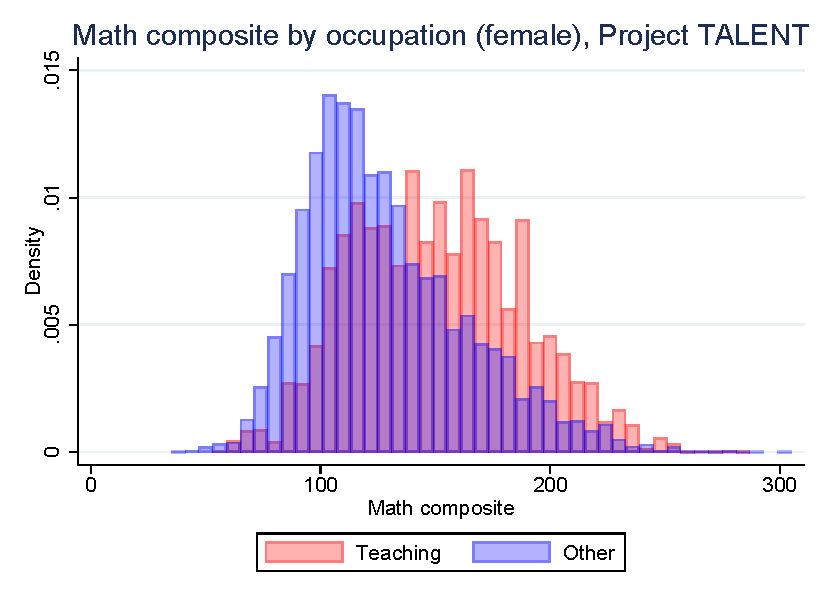
\includegraphics[width=\textwidth]{plots/TALENT_math_occ_no_norm_female_no_lf.pdf}
			\end{subfigure}
			\hfill
			\begin{subfigure}[b]{0.27\textwidth}
				\centering
				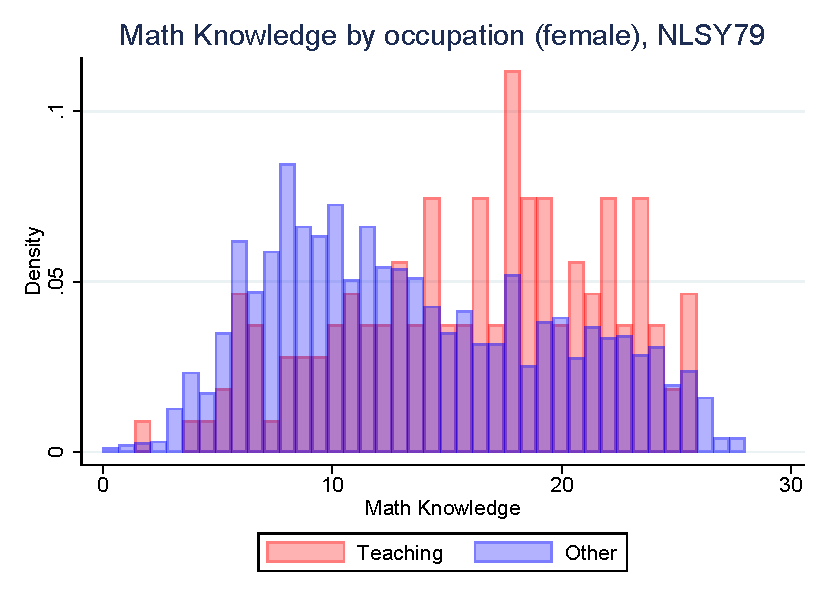
\includegraphics[width=\textwidth]{plots/nlsy79_mk_occ_no_norm_female_no_lf.pdf}
			\end{subfigure}
			\hfill
			\begin{subfigure}[b]{0.27\textwidth}
				\centering
				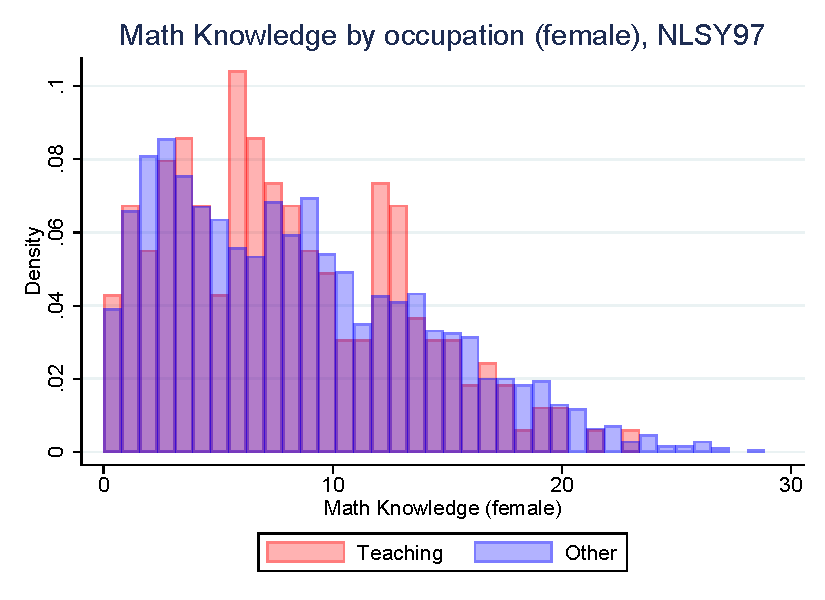
\includegraphics[width=\textwidth]{plots/nlsy97_mk_occ_no_norm_female_no_lf.pdf}
			\end{subfigure}	
			\vfill	
			\begin{subfigure}[b]{0.27\textwidth}
				\centering
				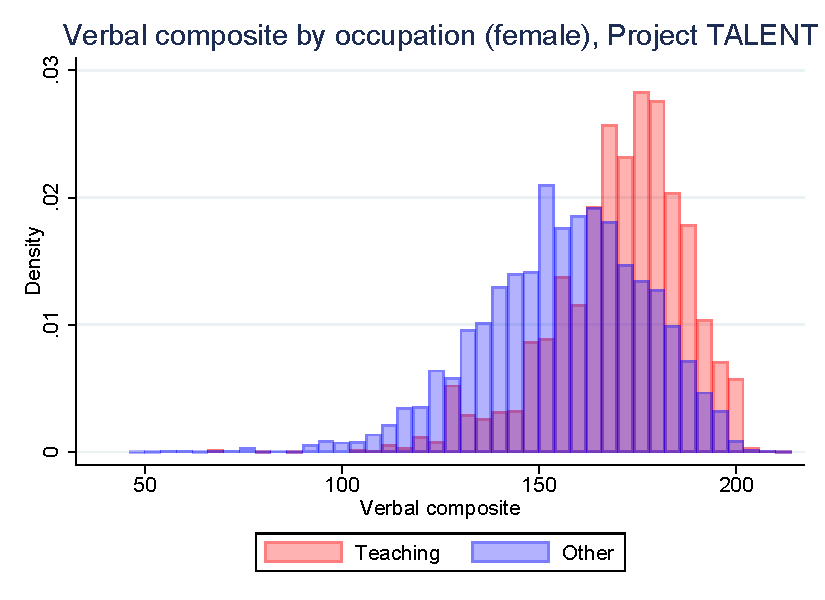
\includegraphics[width=\textwidth]{plots/TALENT_verbal_occ_no_norm_female_no_lf.pdf}
			\end{subfigure}
			\hfill
			\begin{subfigure}[b]{0.27\textwidth}
				\centering
				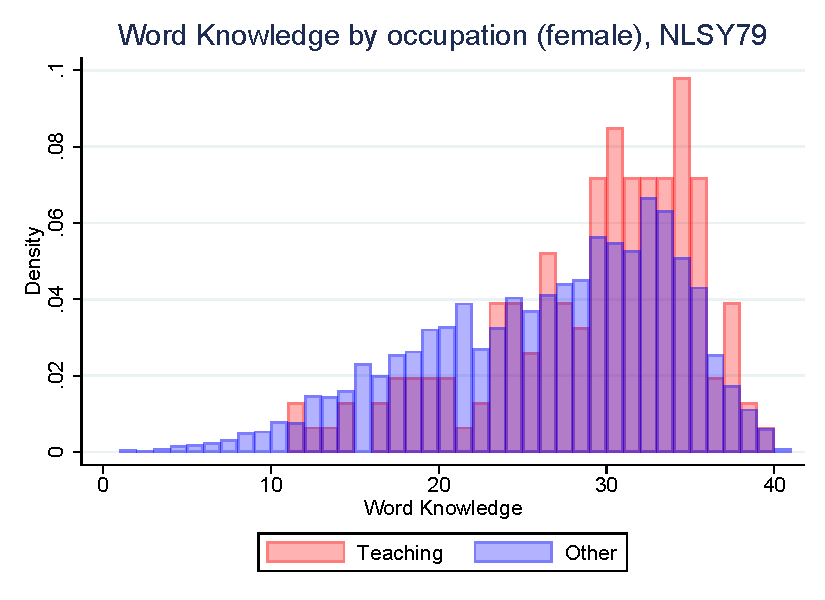
\includegraphics[width=\textwidth]{plots/nlsy79_wk_occ_no_norm_female_no_lf.pdf}
			\end{subfigure}
			\hfill
			\begin{subfigure}[b]{0.27\textwidth}
				\centering
				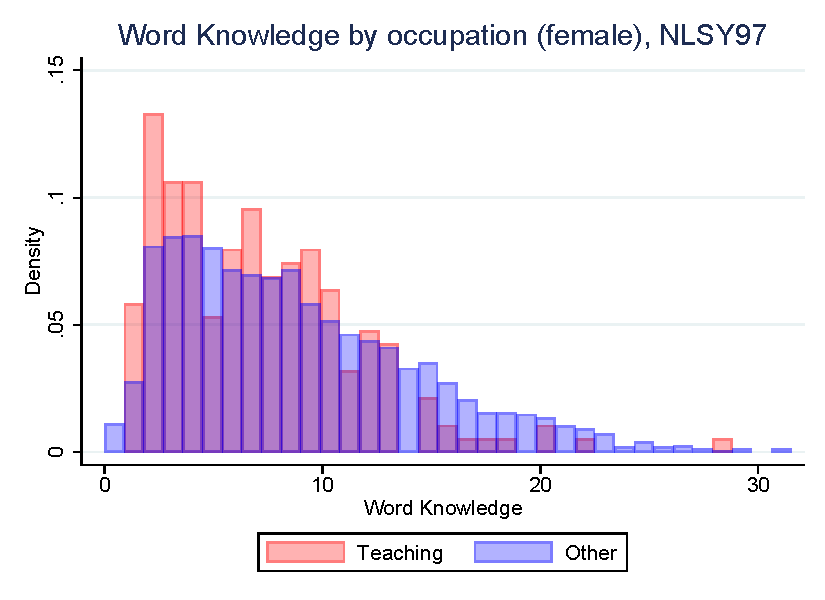
\includegraphics[width=\textwidth]{plots/nlsy97_wk_occ_no_norm_female_no_lf.pdf}
			\end{subfigure}	
		\end{figure}
		\vfill
	\end{adjustwidth}
\end{frame}



%\begin{frame}{}{}
%	\begin{adjustwidth}{2em}{2em}
%		\vfill
%		\begin{figure}[ht!]
%			\begin{subfigure}[b]{0.29\textwidth}
%				\centering
%				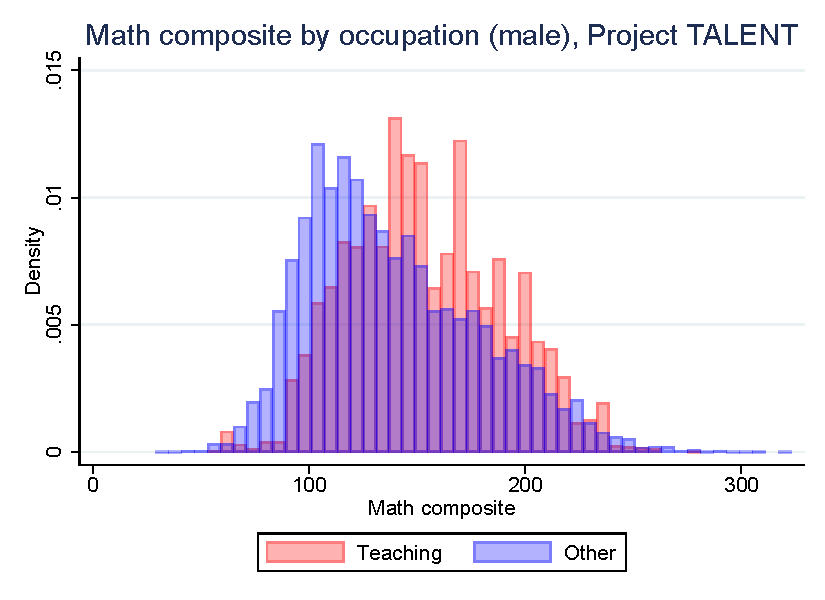
\includegraphics[width=\textwidth]{TALENT_math_occ_no_norm_male_no_lf.pdf}
%			\end{subfigure}
%			\hfill
%			\begin{subfigure}[b]{0.29\textwidth}
%				\centering
%				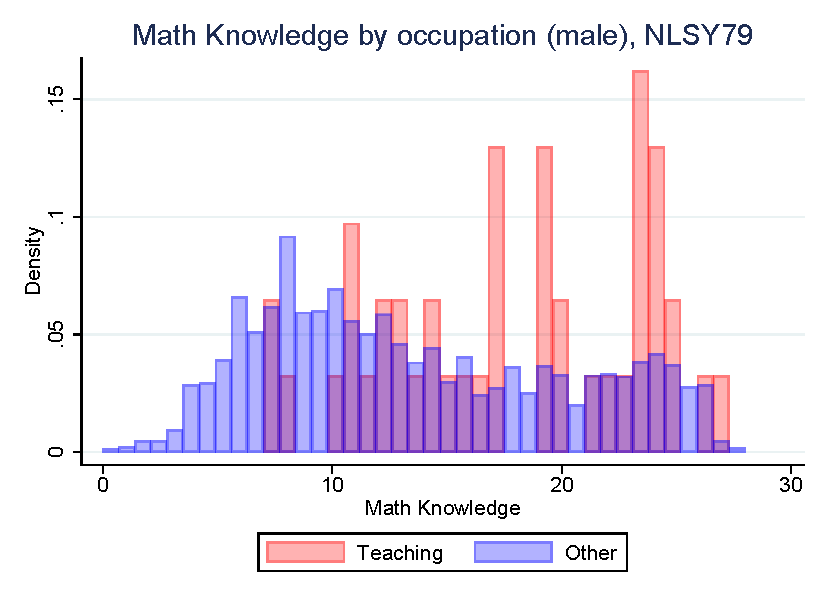
\includegraphics[width=\textwidth]{nlsy79_mk_occ_no_norm_male_no_lf.pdf}
%			\end{subfigure}
%			\hfill
%			\begin{subfigure}[b]{0.29\textwidth}
%				\centering
%				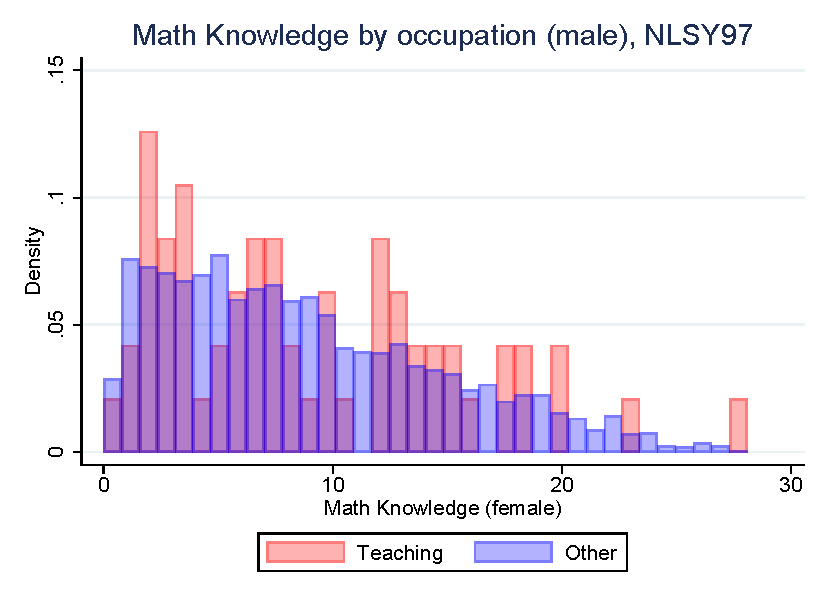
\includegraphics[width=\textwidth]{nlsy97_mk_occ_no_norm_male_no_lf.pdf}
%			\end{subfigure}	
%			\vfill	
%			\begin{subfigure}[b]{0.29\textwidth}
%				\centering
%				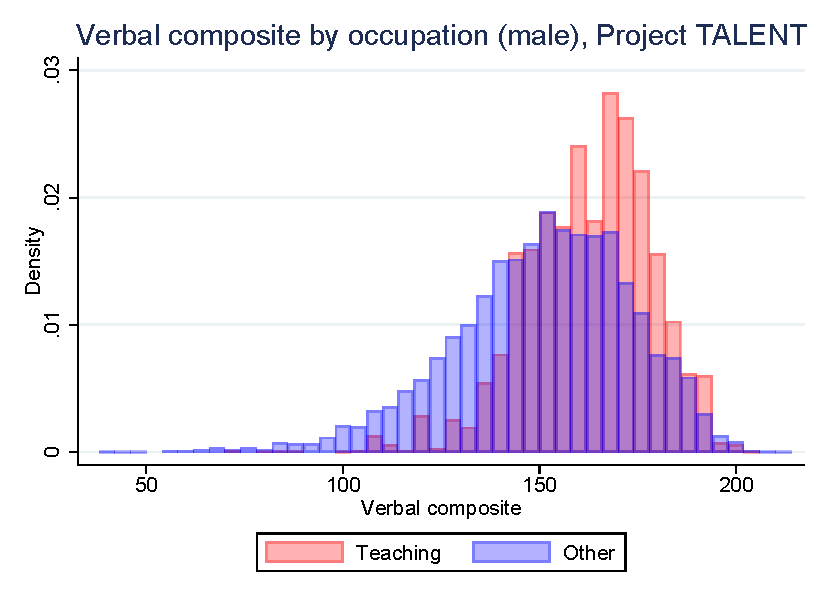
\includegraphics[width=\textwidth]{TALENT_verbal_occ_no_norm_male_no_lf.pdf}
%			\end{subfigure}
%			\hfill
%			\begin{subfigure}[b]{0.29\textwidth}
%				\centering
%				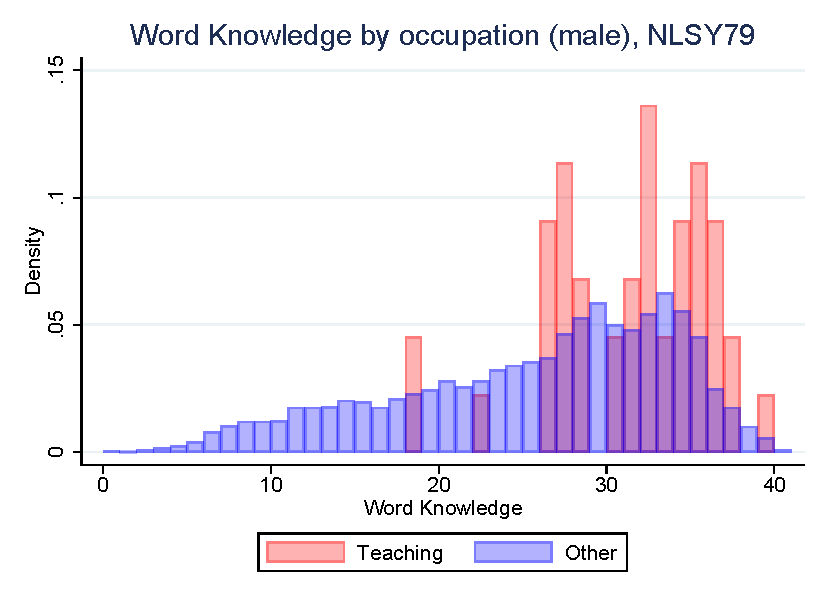
\includegraphics[width=\textwidth]{nlsy79_wk_occ_no_norm_male_no_lf.pdf}
%			\end{subfigure}
%			\hfill
%			\begin{subfigure}[b]{0.29\textwidth}
%				\centering
%				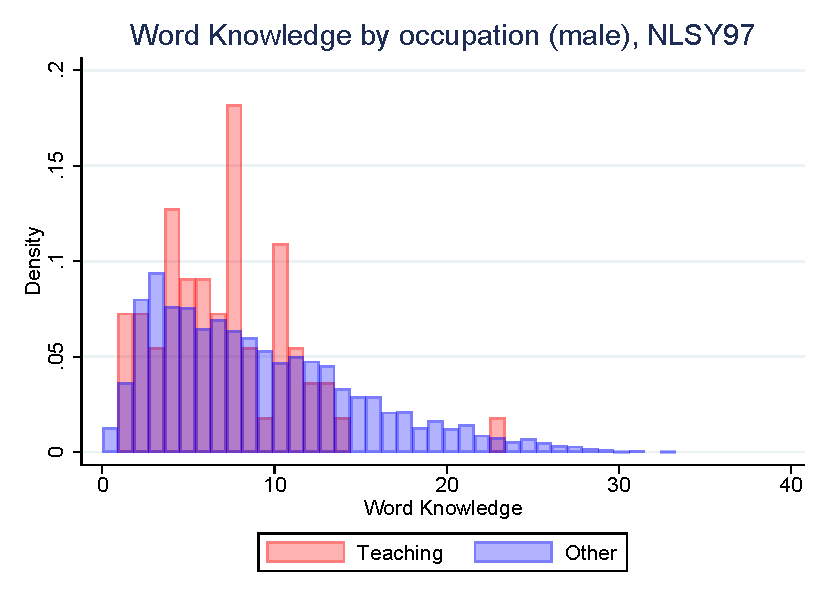
\includegraphics[width=\textwidth]{nlsy97_wk_occ_no_norm_male_no_lf.pdf}
%			\end{subfigure}	
%		\end{figure}
%		\vfill
%	\end{adjustwidth}
%\end{frame}

%\begin{frame}
%\begin{table}[h!]
%		\centering 
%		\begin{tabular}{lccccc}
%			\toprule
%			%\multicolumn{6}{c}{Panel A: 5-Year Post}\\
%			%\midrule
%			% & \multirow{2}{*}{Teachers} & \multirow{2}{*}{Other}& \multirow{2}{*}{Unemployed} & Not in \\
%			% &  & & & Labor Force & \multirow{2}{*}{Total}\\
%			%\midrule
%			%Female & 9,392 & 32,337 & 17,974 & &\\
%			%\quad (\% of subsample) & (74.01\%) & (39.06\%) & (79.46\%) & &\\
%			%\midrule
%			%Math composite mean & 95.31 & 74.10 & 71.94 & &\\
%			%\quad (st.dev.) & (31.78) & (33.43) & (33.19) & &\\
%			%\midrule
%			%Verbal composite mean & 126.26 & 109.63 & 112.67 & &\\
%			%\quad (st.dev.) & (16.44) & (22.09) & (21.08) & &\\
%			%\midrule
%			%Observations & 12,690 & 82,798 & 22,620 & &\\
%			%\quad (\% of total sample) & (10.74\%) & (70.10\%) & (19.15\%) & &\\
%			%\bottomrule
%			%\\
%			%\toprule
%			%\multicolumn{6}{c}{Panel B: 11-Year Post} \\
%			\multicolumn{6}{c}{11-Year Post} \\
%			\midrule
%			& \multirow{2}{*}{Teachers} & \multirow{2}{*}{Other} & \multirow{2}{*}{Unemployed}& Not in \\
%			&  &  & & Labor Force & \multirow{2}{*}{Total}\\
%			\midrule
%			Female & 3,589 & 15,802 & 1,153 & 22,072 & 42,616\\
%			\quad (\% of subsample) & (61.13\%) & (31.24\%) & (62.97\%) & (93.14\%) &(51.36\%)\\
%			\midrule
%			Math composite mean & 157.944 & 147.933 & 142.941 & 139.227 & 146.022\\
%			\quad (st.dev.) & (35.562) & (41.209) & (44.134) & (37.058) & (40.058) \\
%			\midrule
%			Verbal composite mean & 168.815 & 159.736 & 160.062 & 163.336 & 161.433\\
%			\quad (st.dev.) & (15.892) & (20.364) & (22.414) & (18.262) & (19.706)\\
%			\midrule
%			%Social composite mean & 2.915 & 2.660 & 2.563 & 2.753 & 2.703\\
%			%\quad (st.dev.) & (0.988) & (1.000) & (0.985) & (0.996) & (1.0)\\
%			%\midrule
%			%IQ composite mean & 4.330 & 3.964 & 3.887 & 3.978 & 3.992\\
%			%\quad (st.dev.) & (0.822) & (1.027) & (1.128) & (0.955) & (1.0)\\
%			%\midrule
%			Observations & 5,871 & 50,581 & 1,831 & 23,697 & 82,980\\
%			\quad (\% of total sample) & (7.16\%) & (61.70\%) & (2.23\%) & (28.91\%) &(100.0\%)\\
%			\bottomrule
%		\end{tabular}
%		\caption{Project TALENT Test Scores by Occupation}
%		\label{tab:PTscores}
%	\end{table}
%\end{frame}
%
%\begin{frame}
%	\begin{table}[h!]
%		\centering
%		\begin{tabular}{lccccc}
%			\toprule
%%			\toprule
%			\multicolumn{6}{c}{Panel A: NLSY79}\\
%						\midrule
%			& \multirow{2}{*}{Teachers} & \multirow{2}{*}{Other} & \multirow{2}{*}{Unemployed} & Not in & \multirow{2}{*}{Total}\\
%			& &  &  & Labor Force & \\
%			\midrule
%			Female & 153 & 3,101 & 292 & 1,159 & 4,705\\
%			\quad (\% of subsample) & (77.66\%) & (46.11\%) & (50.08\%) & (77.94\%) & (52.32\%)\\
%			\midrule
%			Math knowledge & 16.541 & 13.540 & 10.275 & 10.580 & 12.904\\
%			\quad (st.dev.) & (5.696) & (6.420) & (5.599) & (5.810) & (6.409)\\
%			\midrule
%			Word knowledge & 29.642 & 26.065 & 21.293 & 22.165 &  25.189\\
%			\quad (st.dev.) & (5.969) & (7.920) & (8.751) & (8.980) & (8.335)\\
%			\midrule
%			%Social ability & 3.891 & 3.824 & 3.566 & 3.552 & 3.777\\
%			%\quad (st.dev.) & (1.016) & (0.980) & (0.969) & (1.011) & (1)\\
%		%	\midrule
%		%	AFQT & 1.780 &  1.741 & 1.184 & 1.270 & 1.638\\
%		%	\quad (st.dev.) & (0.928) & (1.004) & (0.950) & (0.956) & (1)\\
%		%	\midrule
%			Observations &  197 & 6,725 & 583 & 1,487 & 8,992\\
%			\quad (\% of total sample) & (2.19\%) & (74.79\%) & (6.48\%) & (16.54\%) & (100.00\%)\\
%			\bottomrule
%%			\bottomrule
%			\\
%			\toprule
%%			\toprule
%			\multicolumn{6}{c}{Panel B: NLSY97}\\
%			\midrule
%			& \multirow{2}{*}{Teachers} & \multirow{2}{*}{Other} & \multirow{2}{*}{Unemployed} & Not in & \multirow{2}{*}{Total}\\
%			& &  &  & Labor Force & \\
%			\midrule
%			Female & 209 & 2,495 & 179 & 327 & 3,062\\
%			\quad (\% of subsample) & (77.41\%) & (46.34\%) & (48.27\%) & (64.53\%) & (50.52\%)\\
%			\midrule
%			Math knowledge & 8.220 & 8.634 & 9.379 & 9.995 & 8.860\\
%			\quad (st.dev.) & (5.339) & (5.840) & (6.408) & (6.521) & (5.979)\\
%			\midrule
%			Word knowledge & 7.068 & 8.965 & 11.745 & 11.493 &  9.415\\
%			\quad (st.dev.) & (4.319) & (5.811) & (6.952) & (6.874) & (6.103)\\
%			\midrule
%		%	Social ability & 5.684 & 5.645 & 5.478 & 5.460 & 5.614\\
%		%	\quad (st.dev.) & (0.904) & (0.967) & (1.108) & (1.158) & (1)\\
%		%	\midrule
%		%	AFQT & 1.776 & 1.665 & 1.045 & 1.185 & 1.585\\
%		%	\quad (st.dev.) & (0.943) & (0.998) & (0.808) & (0.961) & (1)\\
%		%	\midrule
%			Observations &  270 & 4.650 & 346 & 922 & 6,188\\
%			\quad (\% of total sample) & (4.36\%) & (75.15\%) & (5.59\%) & (14.90\%) & (100.00\%)\\
%			\bottomrule
%%			\bottomrule			
%		\end{tabular}
%		\caption{NLSY Scores by Occupation}
%		\label{tab:NLSYscores}
%	\end{table}
%\end{frame}

%\begin{frame}
%\frametitle{Introduction (cont'd)}
%\begin{itemize}
%  \item Broad labor market facts and trends consistent with occupational choice as important mechanism:
%  \begin{itemize} \pause
%  \item Female educational attainment rising
%  \item Female labor force participation rising
%  \item Labor market discrimination against women declining (Hsieh et al., 2019)
%  \item U.S. public school teachers largely female
%\end{itemize} \pause
%  \item Static gains vs. dynamic associated with departure of high-ability female teachers? 
%\end{itemize}
%\end{frame}

\begin{frame}

\end{frame}

\begin{frame}
\frametitle{Model}
\framesubtitle{Endowments, Preferences}
\begin{itemize}
  \item Each period, a measure $M$ of agents is born and lives for two periods (``young'' and ``old'')
%  \item Individuals born with occupation-specific abilities drawn from a joint bivariate Fr\'echet distribution with c.d.f.
  \item Individuals born with occupation-specific abilities drawn from a joint bivariate distribution with c.d.f. $F(a^T,a^O)$
%  \begin{equation*}
%\label{ }
%F(a^T,a^O) = \exp \left[ - a_T^{-\theta} - a_O^{-\theta} \right],
%\end{equation*}
%  \item Individuals live for two periods labeled ``young'' and ``old'' and economy populated by two overlapping generations
  \item Individuals have $\log$ preferences over leisure and consumption (no discounting):
  \begin{displaymath}
\ln c_{t+1} + \ln\left(1-s_t\right)
\end{displaymath}
\end{itemize}
\end{frame}

\begin{frame}
\frametitle{Model}
\framesubtitle{Technologies}
\begin{itemize}
  \item Children (``young'') make occupation-specific educational investments (in units of time and output)
  \item Adults work as \alert{teachers} or \alert{production workers}.
%  \item Technologies are occupation-specific:
  \begin{description}
  \item[Human capital production] (teaching) depends on teacher's $h^T$, child's ability $a$, and child's educational investments (time $s$ and goods $e$) according to:
  \begin{align*}
\label{}
h^{'}(a) & = \left( h^T\right)^\beta a^\alpha s\left(a\right)^\phi e(a)^\eta {N(h^T,\widetilde{H}^T)}^{-\sigma} \\
& \textrm{{\sf where }} \widetilde{H}^T = \int_0^\infty \left( h^T\left( a \right) \right)^{\frac{\beta}{\sigma}} f^T(a) da
\end{align*}
  \item[Final output production] depends on adult worker's human capital $h^O$ and exogenous productivity $A^O$:
    \begin{align*}
\label{}
y = A^O h^O
\end{align*}
\end{description}
\end{itemize}
\end{frame}


\begin{frame}
\frametitle{Model}
\framesubtitle{Values}
\begin{align*}
V^g(a^T,a^O,\widetilde{H}^T) & = \max_{\{s^{O},s^{T},e^{O},e^{T}\}} \bigg\{ V^{O,g}(a^O,\widetilde{H}^T), V^{T,g}(a^T,\widetilde{H}^T) \bigg\}
\end{align*}
where
\begin{align*}
%\label{eq:vo}
V^{O,g}(a^O,\widetilde{H}^T) & = \ln\left(1-s^O\left(a^O,\widetilde{H}^T\right)\right) \\
& + \mu \ln \Big[ {{h'}^{O}} {A'}^O(1-{{\tau'}^{O,g,w}})\alert{(1-t)} \\
& - e^O(a^O,\widetilde{H}^T)(1+\tau^{O,g,e}) \Big],  \\
%\label{eq:vt}
V^{T,g}(a^T,\widetilde{H}^T) & = \ln\left(1-s^T\left(a^T,\widetilde{H}^T\right)\right)  \\
& + \mu \ln \Big[ \omega'({{h'}^{T}},{\widetilde{H'}^{T}})(1-{{\tau'}^{T,g,w}})\alert{(1-t)}  \\
& - e^T(a^T,\widetilde{H}^T)(1+\tau^{T,g,e}) \Big] 
\end{align*}
\end{frame}

\begin{frame}
\frametitle{Model (cont'd)}
\framesubtitle{Constraints, Laws of Motion}
\begin{align}
%H^{T} & = \int_{0}^{\infty} \left(h^{T}(a)\right)^{\frac{\beta}{\sigma}} f^{T}(a) da \\
\alert{t}  \int_0^\infty \big( \omega\left(h^{T}\left( a \right) \right) {f}^T(a) & + A^O h^O(a) f^O(a) \big) da  = \int_0^\infty \omega\left(h^{T}(a)\right) {f}^T(a) da \nonumber\\%\frac{2}{M} \int_0^\infty \omega\left(h^{T'}(a)\right) {f'}^T(a) da \nonumber\\
%\label{eq:densT}
f^T(a) & = \int_0^{\bar{a}^{-1}\left(a\right)} f\big(a,b \big) db \nonumber\\
%\label{eq:densO}
f^O(b) & = \int_0^{\bar{a}\left(b\right)} f\big(a,b \big) da \nonumber
%f^T(a) & = \int_0^{\bar{a}\big(a;H^T,{H^T}'\big)} f\big(a,a^O\big) da^O 
\end{align}
Aggregate laws of motion for $\widetilde{H}^T$ and ${H}^O$:
\begin{align}
%\label{eq:lomT}
\widetilde{H'}^{T} & = \int_0^\infty \left(\left(\tfrac{2 \widetilde{H}^T}{M}\right)^\sigma a^\alpha s^T\left(a,\widetilde{H}^T\right)^\phi e^T(a,\widetilde{H}^T)^\eta \right)^{\frac{\beta}{\sigma}} f^T(a) da \nonumber \\
%\label{eq:lomO}
{H'}^{O} & = \int_0^\infty \left(\tfrac{2 \widetilde{H}^T}{M}\right)^\sigma a^\alpha s^O\left(a,\widetilde{H}^T\right)^\phi e^O(a,\widetilde{H}^T)^\eta  f^O(a) da \nonumber
\end{align}
\end{frame}

\begin{frame}
\frametitle{Model (cont'd)}
\framesubtitle{Occupational Threshold}
%Idiosyncratic human capital investment technology:
%\begin{align*}
%\label{}
%h^{O'}(a^O) & = \left(\frac{2 H^T}{M}\right)^\sigma \left(a^O\right)^\alpha s^O\left(a^{O},H^T,{H^T}'\right)^\phi e^O(a^{O},H^T,{H^T}')^\eta \\
%h^{T'}(a^T) & = \left(\frac{2 H^T}{M}\right)^\sigma \left(a^T\right)^\alpha s^T\left(a^{T},H^T,{H^T}'\right)^\phi e^T(a^{T},H^T,{H^T}')^\eta
%\end{align*}
%Occupational threshold:
\begin{equation*}
%\label{eq:ot}
a^{T*}(a^O) = \bar{a}\big(a^{O},\widetilde{H}^T\big) %\\
\end{equation*}
such that
\begin{equation*}
V^{O}(a^{O},\widetilde{H}^T) = V^{T}\left(a^{T*}(a^O),\widetilde{H}^T\right) \textrm{{\sf , for all} } a^O \in (0,\infty)
\end{equation*}

\end{frame}

\begin{frame}
\frametitle{Model (cont'd)}
%\begin{description}
%  \item[Problem \#1:] We don't know $\omega(\cdot,\cdot)$ and we need to compute it numerically!
%  \item[Challenge:] $\omega(\cdot,\cdot)$ is possibly non-linear in $h^T$ (for given $H^T$) 
%  \item[Problem \#2:] For given $\omega(\cdot,\cdot)$, need to identify the fixed point $H^{T'} = {\widetilde{H^{T'}}} $.
%  \item[Solution:] $\omega(\cdot,\cdot)$ is proportional to the \textit{number of students} in a teacher's class:
%  \begin{equation*}
%\omega(h^T,H^T) = \lambda N(h^T,H^T) = \lambda \frac{M}{2 H^T} \left( h^T \right)^{\frac{\beta}{\sigma}}
%\end{equation*}
\begin{itemize}
  \item Assignment of students to teachers is random \\ $\Rightarrow$ distribution of students' skill identical across classrooms
  \item Teachers with different $h^T$ vary with respect to class {\it size}
  \item $\omega(\cdot,\cdot)$ is proportional to the \textit{number of students} in a teacher's class and to :
  \begin{align*}
\omega(h^T,\widetilde{H}^T) & = \lambda N(h^T,\widetilde{H}^T) \\
& = \frac{{H'}^O {A'}^O}{\frac{M}{2}\int_o^\infty f^O(a) da} \underbrace{\overbrace{N(1,\widetilde{H}^T)}^{=\frac{M}{2}\frac{1}{\widetilde{H}^T}}\left( h^T \right)^{\frac{\beta}{\sigma}}}_{=N(h^T,\widetilde{H}^T)} \\
& = \frac{{H'}^O {A'}^O}{\int_o^\infty f^O(a) da} \frac{\left( h^T \right)^{\frac{\beta}{\sigma}}}{{\widetilde{H}^T}}
\end{align*}
%  \item $\lambda$ is the value of human capital per worker (in units of output) in occupation $O$.
\end{itemize}

%  \item[Implication:] standard Roy model results no longer hold
%\end{description}
\end{frame}

\begin{frame}
\frametitle{Optimal Investments for Prospective Teachers (I)} 
%The F.O.C.s for $s^T$ and $e^T$, respectively, after a few steps of algebra are:
\begin{align}
%\label{eq:s_T}
s^{T} & = \frac{\mu \phi}{\mu \phi+\frac{\beta}{\sigma}-\eta} \nonumber\\
%\label{eq:e_T}
e^{T} & = \left( \frac{(1-t)(1-{\tau'}^{T,w})\left(\tfrac{2}{M}\right)^\beta {A'}^O (s^{T})^\frac{\phi \beta}{\sigma} \left(\tfrac{\eta \beta}{\sigma}\right) \left(\alert{\widetilde{H}^T}\right)^\beta \left(a^{T}\right)^\frac{\alpha \beta}{\sigma}}{1+\tau^{T,e}} \right)^\frac{1}{1-\frac{\eta\beta}{\sigma}} \nonumber\\
& \times \left(\frac{\alert{{H'}^O}}{\int_o^\infty f^O(a) da}\left(\alert{\widetilde{H'}^{T}}\right)^{-1}\right)^\frac{1}{1-\frac{\eta\beta}{\sigma}} \nonumber
\end{align}
%where
%\begin{align}
%\eta\beta < \sigma \nonumber
%\label{}
% \frac{\partial \omega'}{\partial s^T} & =  \frac{\beta \phi}{\sigma} \lambda' \left(\frac{M}{2 H^T}\right)^{-\beta} \frac{M}{2 {{H'}^T}} \left[ a^\alpha (s^T)^\phi (e^T)^\eta \right]^{\frac{\beta}{\sigma}} \frac{1}{s^T} \nonumber \\
% \frac{\partial \omega'}{\partial e^T} & = \frac{\beta \eta}{\sigma} \lambda' \left(\frac{M}{2 H^T}\right)^{-\beta} \frac{M}{2 {{H'}^T}} \left[ a^\alpha (s^T)^\phi (e^T)^\eta \right]^{\frac{\beta}{\sigma}} \frac{1}{e^T} \nonumber
%\end{align}
\end{frame}

\begin{frame}
\frametitle{Aggregate Laws of Motion} 
\begin{align}
%\label{eq:lomT}
\widetilde{H'}^{T} & = \Bigg[ \left(\frac{(1-{\tau'}^{T,w})\left(\tfrac{\eta \beta}{\sigma}\right)}{1+\tau^{T,e}} \right)^\eta \left(\frac{(1-{\tau'}^{O,w}) \eta}{1+\tau^{O,e}} \right)^{\frac{\eta}{1-\eta} \eta} \left((1-t){A'}^O \right)^\frac{\eta}{1-\eta}\nonumber\\
& \times  \left(\frac{2}{M}\right)^\frac{\sigma}{1-\eta} (s^{T})^\phi (s^{O})^{\frac{\eta}{1-\eta}\phi} \left(\frac{\int_0^\infty a^\frac{\alpha}{1-\eta} f^O(a) da}{\int_0^\infty f^O(a) da} \right)^\eta
 \nonumber\\
& \times  \left(\int_0^\infty a^\frac{\alpha\beta}{\sigma-\eta\beta} f^T(a) da\right)^{\frac{\sigma-\eta\beta}{\beta}} \left(\widetilde{H}^T\right)^{\alert{\frac{\sigma}{1-\eta}}} \Bigg]^{\alert{\frac{\beta}{\sigma}}} \nonumber\\
%\label{eq:lomO}
{H'}^{O} & = \left( \frac{(1-t)(1-{\tau'}^{O,w}){A'}^O \eta}{1+\tau^{O,e}}\right)^{\frac{\eta}{1-\eta}} \left(\frac{2}{M}\right)^\frac{\sigma}{1-\eta} (s^{O})^\frac{\phi}{1-\eta} \nonumber\\
& \times \left(\int_0^\infty a^\frac{\alpha}{1-\eta} f^O(a) da\right) \left(\widetilde{H}^T\right)^\frac{\sigma}{1-\eta} \nonumber
%\int_0^\infty \left(\tfrac{2 \widetilde{H}^T}{M}\right)^\sigma a^\alpha s^O\left(a,\widetilde{H}^T\right)^\phi e^O(a,\widetilde{H}^T)^\eta  f^O(a) da \nonumber
\end{align}
\end{frame}

\begin{frame}
\frametitle{Optimal Investments for Prospective Teachers (II)} 
\begin{align}
%\label{eq:s_T}
s^{T} & = \frac{\mu \phi}{\mu \phi+\frac{\beta}{\sigma}-\eta} \nonumber\\
%\label{eq:e_T}
e^{T} & = \left( (1-t) \left(\tfrac{2}{M}\right)^\sigma {A'}^O \eta (s^{O})^\phi \alert{\left(\widetilde{H}^T\right)^\sigma} \left(a^{T}\right)^\alpha\right)^{\alert{\frac{1}{1-\eta}}} \nonumber\\
& \times \frac{(1-{\tau'}^{T,w})(1-{\tau'}^{O,w})^\frac{\eta}{1-\eta}}{(1+{\tau}^{T,e})(1+{\tau}^{O,e})^\frac{\eta}{1-\eta}} \cdot \frac{\beta}{\sigma} \nonumber\\
& \times \left( \frac{\int_0^\infty a^\frac{\alpha}{1-\eta} f^O(a) da}{\int_0^\infty f^O(a) da}\right) \left( \int_0^\infty a^\frac{\alpha}{\frac{\sigma}{\beta}-\eta} f^T(a) da \right)^{-1} \nonumber
\end{align}

\end{frame}

\begin{frame}
\frametitle{Optimal Investments for Prospective ``Other'' Workers} 
%The F.O.C.s for $s^O$ and $e^O$ are, respectively:
\begin{align}
%\label{eq:s_O}
s^{O} & = \frac{\mu \phi}{\mu \phi+1-\eta} \nonumber \\
%\label{eq:e_O}
e^{O} & = \left( \frac{(1-t)(1-{\tau'}^{O,w})\left(\tfrac{2}{M}\right)^\sigma {A'}^O (s^{O})^\phi \eta \left(\widetilde{H}^T\right)^\sigma \left(a^{O}\right)^\alpha}{1+\tau^{O,e}} \right)^\frac{1}{1-\eta} \nonumber
\end{align}
%where
%\begin{align}
%\eta < 1  \nonumber
%\end{align}
\end{frame}

\begin{frame}
\frametitle{Some Parameter Restrictions}
\begin{itemize}
  \item $\beta < 1-\eta$ to guarantee existence of stable $\widetilde{H^T} = \widetilde{H^T}' > 0$
  \item $\tfrac{\sigma}{\beta} > \eta$ and $\mu \phi > 0$ for $s^{T*} \in (0,1)$
  \item $1 > \eta$ and $\mu \phi > 0$ for $s^{O*} \in (0,1)$
\end{itemize}
\end{frame}

%\begin{frame}
%\frametitle{Aggregate laws of motion (cont'd)} 
%There exist a strictly positive, stable fixed point in $\widetilde{H}^T$ if:
%\begin{equation*}
%\beta<1-\eta
%\end{equation*}
%\end{frame}

\begin{frame}
\frametitle{Occupational Choice Boundary\ldots}
\framesubtitle{\ldots does not depend on aggregate state $\widetilde{H^T}$} 
\begin{align}
\left(\frac{1-{\tau'}^{O,w}}{1-{\tau'}^{T,w}}\right) \left(\frac{1-\eta}{1-\tfrac{\eta\beta}{\sigma}}\right)  \left(\frac{1-s^{O}}{1-s^{T}}\right)^{\frac{1}{\mu}}  \left(\frac{(a^O)^\frac{\alpha}{1-\eta}}{\big(\alert{\bar{a}^T(a^O)}\big)^\frac{\alpha}{\frac{\sigma}{\beta}-\eta}} \right) \nonumber\\
= \left(\frac{\int_0^\infty a^\frac{\alpha}{1-\eta} \alert{f^O(a)} da}{\int_0^\infty \alert{f^O(a)} da} \right) \left(\int_0^\infty a^\frac{\alpha}{\frac{\sigma}{\beta}-\eta} \alert{f^T(a)} da\right)^{-1} \nonumber
\end{align}
\end{frame}

\begin{frame}
\frametitle{Equilibrium}
% Definition with references:
%The equilibrium is characterized by the F.O.C.s \eqref{eq:foc-e} and \eqref{eq:foc-s}, the aggregate laws of motion \eqref{eq:lomT}, the occupational choice boundary \eqref{eq:ot}, the corresponding densities \eqref{eq:densT} and \eqref{eq:densO}, as well as the F.O.C.s for $s$ and $e$ for prospective ``other'' workers (not shown).
% Definition without references:
The equilibrium is characterized by:
\begin{enumerate}
  \item the optimal investment for prospective teachers 
  \item the optimal investment for prospective ``other'' workers
  \item the aggregate laws of motion
  \item the occupational choice boundary and the corresponding densities $f^T$ and $f^O$
\end{enumerate}
\end{frame}

\begin{frame}
\frametitle{Data for Quantitative Exercise}
%\framesubtitle{}
\begin{itemize}
  \item Micro-data on abilities and occupational choice:
\begin{enumerate}
  \item Project TALENT (1960-1975):
  \begin{itemize}
  \item representative 5\% sample of high school population in 1960
  \item follow-up surveys at 1, 5, and 11-year post graduation
\end{itemize}
  \item NLSY 79
  \item NLSY 97
\end{enumerate}
  \item Cognitive abilities in math, verbal,\ldots based on standardized assessments (e.g.~ASVAB in NLSY)
  \item Occupational choice 11 years after (likely) high school graduation in all surveys
\end{itemize}
\end{frame}

\begin{frame}
\frametitle{Occupational Skills from Cognitive Scores}
%\framesubtitle{}
\begin{itemize}
  \item Harmonized cognitive scores from NLSY79 and NLSY97 for:
  \begin{enumerate}
  \item Mathematics knowledge
  \item Arithmetic reasoning
  \item Word knowledge
  \item Paragraph comprehension
\end{enumerate}
  \item ``Crosswalk'' from composite math and verbal scores in Project TALENT to AFQT equivalents (Air Force)
  \item Skill requirements by occupation from O*NET
  \item Occupation-specific skills based on ``translation'' of cognitive scores \alert{(work in progress)}
  \item In contrast to standard Roy model, occupational choice depends on {\it comparative} \alert{and} {\it absolute} advantage here!
\end{itemize}
\end{frame}

\begin{frame}
\frametitle{Ongoing and Future Work}
%\framesubtitle{}
\begin{itemize}
  \item Decentralized equilibrium vs.~planner's solution (human capital externality in teaching)
  \item Calibrated reduction in discrimination \& barriers: \\ static gains (as in Hsieh et al., 2019) vs.~dynamic effects (human capital accumulation)
  \item Multiple locations differentiated by amenities and/or local tax rates (implicit school segregation by income)
\end{itemize}
\end{frame}

%\begin{frame}
%\frametitle{Conclusion}
%
%\end{frame}
%\begin{frame}
%\frametitle{Occupational Threshold}
%\framesubtitle{Variation in Strength of Superstar Effect in Teaching: $\frac{\beta}{\sigma}$}
%\begin{figure}
%\begin{center}
%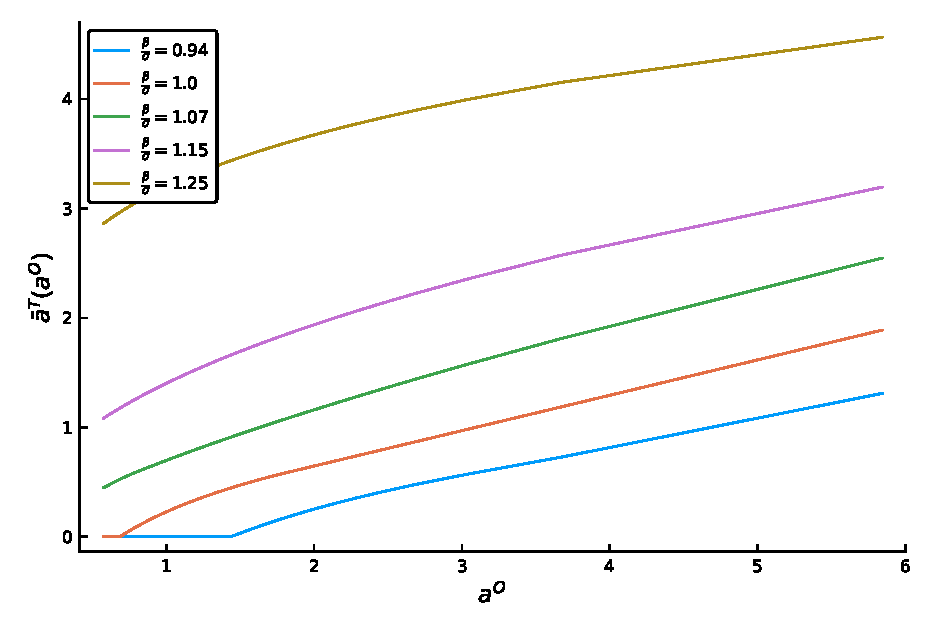
\includegraphics[width=.9\textwidth]{/Users/simeonalder/Dropbox/Work/Research/GitHub/teachers/julia/plots/occ_thresh_tauW_0.0_tauE_0.0_A=2.0.eps}
%%\caption{ }
%%\label{ }
%\end{center}
%\end{figure}
%\end{frame}
%
%\begin{frame}
%\frametitle{Occupational Choice (Aggregate)}
%\framesubtitle{Variation in Strength of Superstar Effect in Teaching: $\frac{\beta}{\sigma}$}
%\begin{figure}
%\begin{center}
%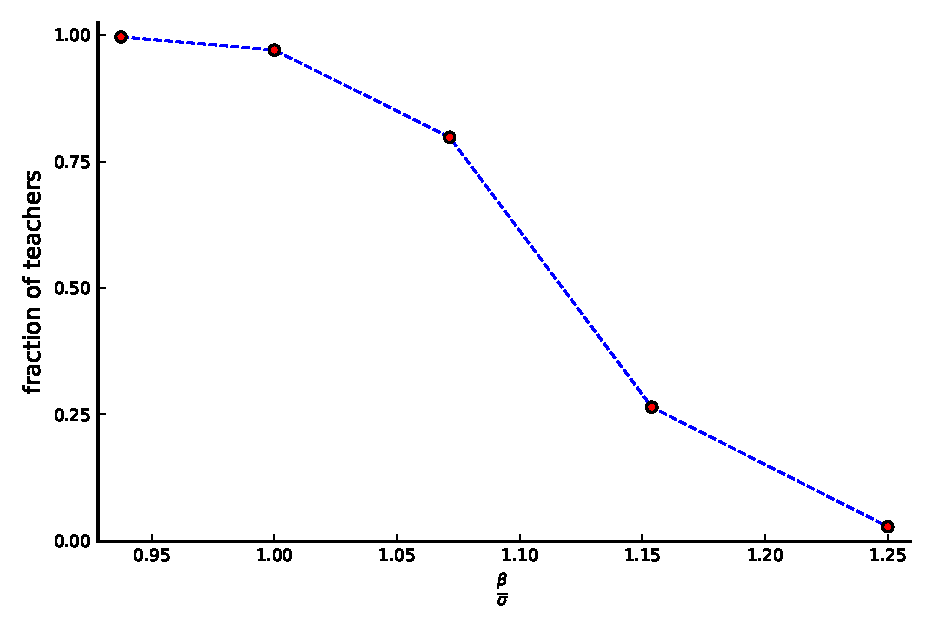
\includegraphics[width=.9\textwidth]{/Users/simeonalder/Dropbox/Work/Research/GitHub/teachers/julia/plots/frac_teachers_tauW_0.0_tauE_0.0_A=2.0.eps}
%%\caption{ }
%%\label{ }
%\end{center}
%\end{figure}
%\end{frame}
%
%\begin{frame}
%\frametitle{Occupational Split}
%\framesubtitle{Variation in Strength of Superstar Effect in Teaching: $\frac{\beta}{\sigma}$}
%\begin{figure}
%\begin{center}
%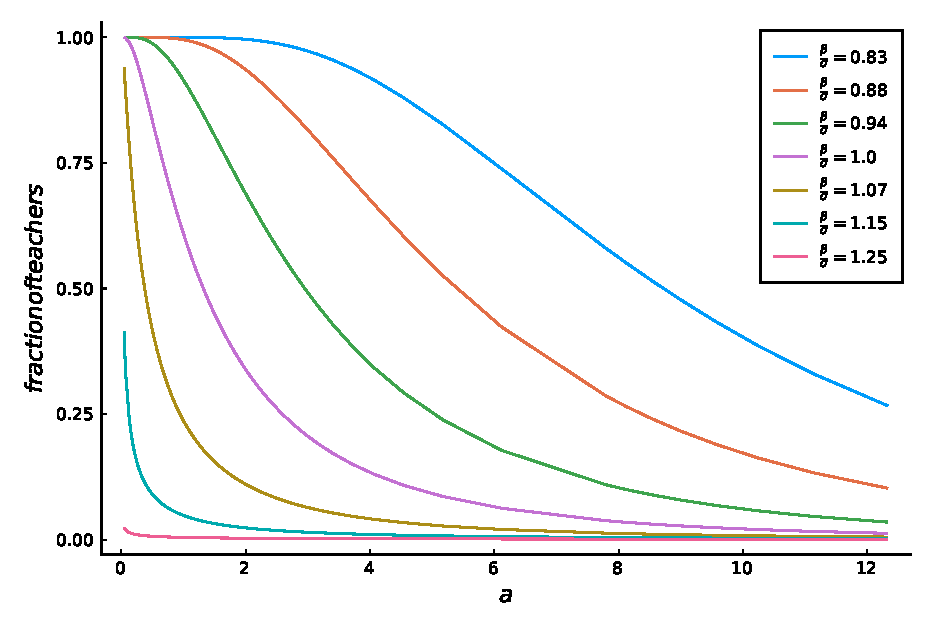
\includegraphics[width=.9\textwidth]{/Users/simeonalder/Dropbox/Work/Research/GitHub/teachers/julia/plots/frac_teachers_by_a_tauW_0.0_tauE_0.0_A=2.0.eps}
%%\caption{ }
%%\label{ }
%\end{center}
%\end{figure}
%\end{frame}
%
%\begin{frame}
%\frametitle{Aggregate Law of Motion for $\widetilde{H^T}$}
%\framesubtitle{Variation in Strength of Superstar Effect in Teaching: $\frac{\beta}{\sigma}$}
%\begin{figure}
%\begin{center}
%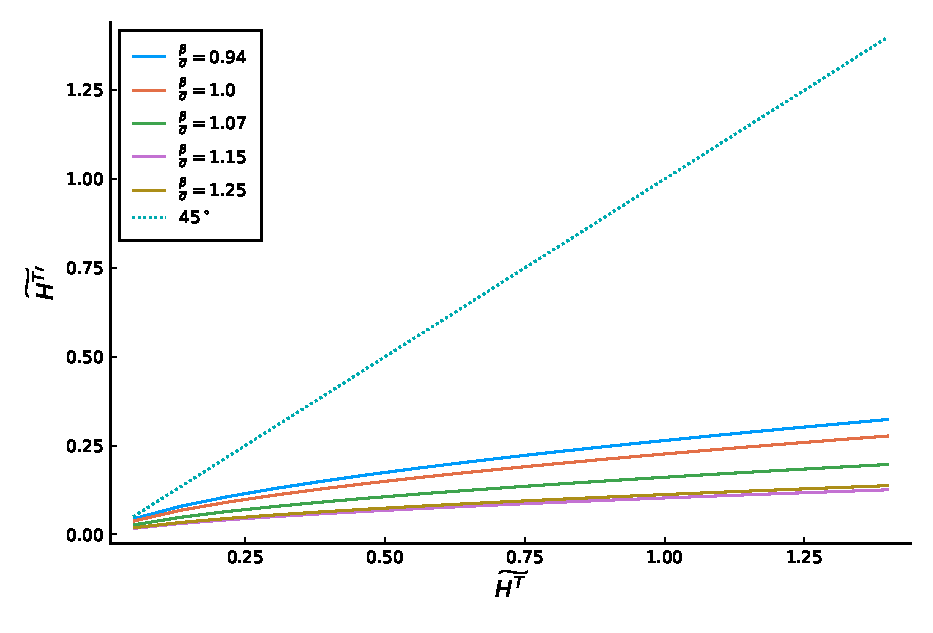
\includegraphics[width=.9\textwidth]{/Users/simeonalder/Dropbox/Work/Research/GitHub/teachers/julia/plots/law_of_motion_tauW_0.0_tauE_0.0_A=2.0.eps}
%%\caption{ }
%%\label{ }
%\end{center}
%\end{figure}
%\end{frame}
%
%\begin{frame}
%\frametitle{Effect of $\tau^w$ on Occupational Choice}
%\framesubtitle{$\frac{\beta}{\sigma} = 1.15$}
%\begin{figure}
%\begin{center}
%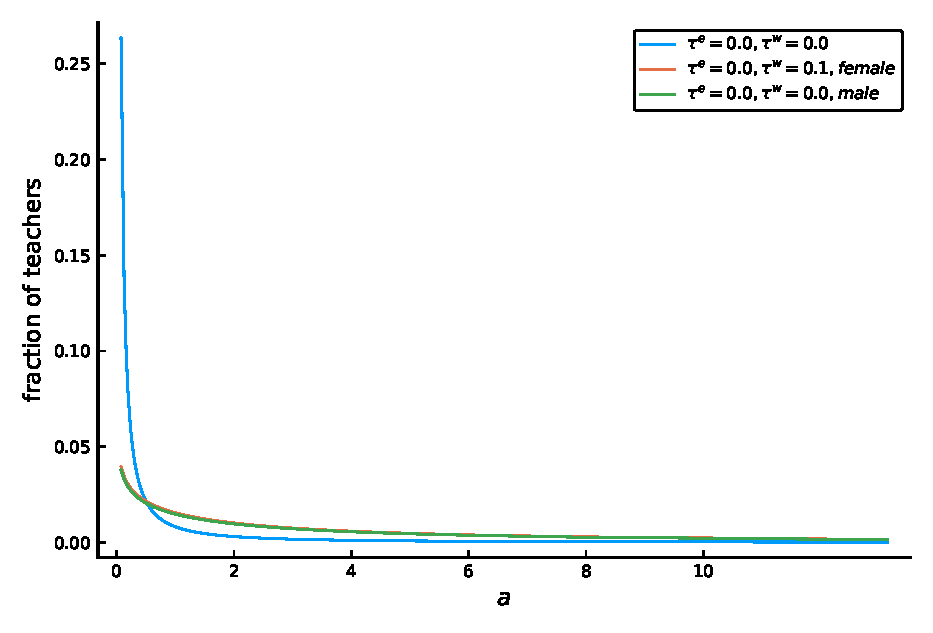
\includegraphics[width=.9\textwidth]{/Users/simeonalder/Dropbox/Work/Research/GitHub/teachers/julia/plots/frac_teachers_by_a_tauW_0.1_tauE_0.0_A=2.0.eps}
%%\caption{ }
%%\label{ }
%\end{center}
%\end{figure}
%\end{frame}
%
%\begin{frame}
%\frametitle{Effect of $\tau^e$ on Occupational Choice}
%\framesubtitle{$\frac{\beta}{\sigma} = 1.15$}
%\begin{figure}
%\begin{center}
%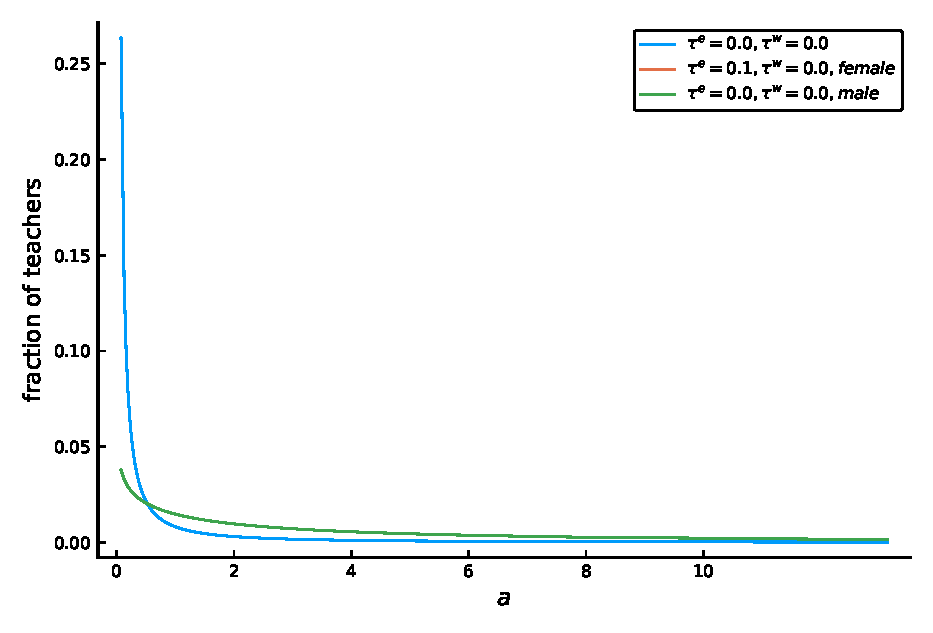
\includegraphics[width=.9\textwidth]{/Users/simeonalder/Dropbox/Work/Research/GitHub/teachers/julia/plots/frac_teachers_by_a_tauW_0.0_tauE_0.1_A=2.0.eps}
%%\caption{ }
%%\label{ }
%\end{center}
%\end{figure}
%\end{frame}
%
%\begin{frame}
%\frametitle{Combined Effect of $\tau^w$ and $\tau^e$ on Occupational Choice}
%\framesubtitle{$\frac{\beta}{\sigma} = 1.15$}
%\begin{figure}
%\begin{center}
%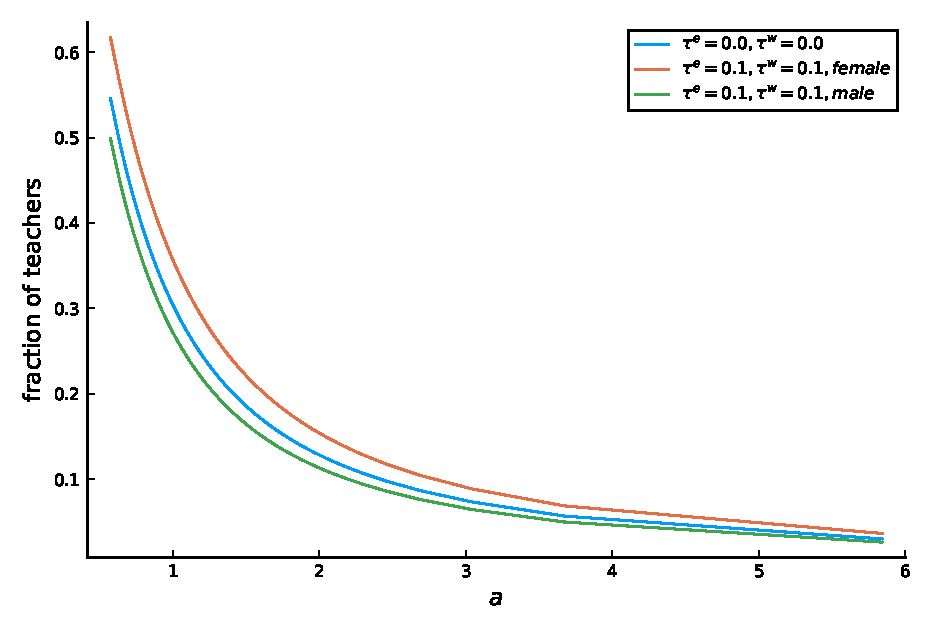
\includegraphics[width=.9\textwidth]{/Users/simeonalder/Dropbox/Work/Research/GitHub/teachers/julia/plots/frac_teachers_by_a_tauW_0.1_tauE_0.1_A=2.0.eps}
%%\caption{ }
%%\label{ }
%\end{center}
%\end{figure}
%\end{frame}

%\begin{frame}
%\frametitle{Extensions}
%\begin{itemize}
%  \item Multiple locations:
%  \begin{itemize}
%  \item finite number of locations
%  \item teachers' salaries funded by combination of local lump-sum (property) and proportional (sales) taxes
%  \item one location with $T=0$, all locations have $t \in (0,1)$
%  \item sorting of teachers and children into locations (high wage = high tax)
%  \item sorting breaks global monotonicity between teacher's $h^T$ and class size (still holds locally, with random within-district assignment)
%  \item to start with, solve with two locations (``high vs.~low'') 
%  \end{itemize}
%\end{itemize}
%\end{frame}

\end{document}